\subsubsection{Umstellen auf Sticky secure MAC addresses}
\begin{figure}[!htb]
    \centering
    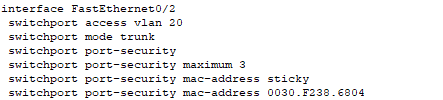
\includegraphics[width=.95\textwidth,keepaspectratio]{./img/config/sticky/config.png}
    \caption{Switch 1 Fa0/2 nach Shutdown}
\end{figure}
\subsubsection{Frage 4}
\paragraph{Frage}
Worin besteht der Unterschied zum Default Verfahren (also ohne
Verwendung von „Sticky secure“ Lernen)?
\paragraph{Antwort}
Beim Default Verfahren sind die Addressen statisch, aber werden auf dem jeweiligen Interface nicht gespeichert. Beim "Sticky secure" wird die Addresse jedoch vom Switch gespeichert und eingetragen.
\begin{figure}[!htb]
    \centering
    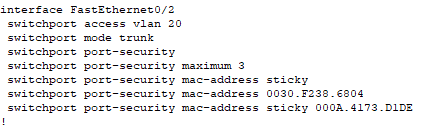
\includegraphics[width=.95\textwidth,keepaspectratio]{./img/config/sticky/result.png}
    \caption{Running Config nach einem Ping}
\end{figure}